\chapter{A função \texorpdfstring{$\zeta$}{zeta} de Riemann}
\chaptermark{}

\hfill%
\begin{minipage}{10cm}
    \begin{flushright}
    \rightskip=0.5cm
        \textit{%
            ``If I were to awaken after having slept for a thousand years, my first question would be: Has the Riemann hypothesis been proven?''
        }
        \\[0.1cm]
    \rightskip=0.5cm
    --- David Hilbert
    \end{flushright}
\end{minipage}

\section{Funções Inteiras}
    \subsection{Fórmula de Jensen e número de zeros}
    
    Nesta seção, mostraremos o Teorema da Fórmula de Jensen, que relaciona os zeros 
    de uma função em um disco com a média logarítmica do módulo desta função ao 
    longo do bordo do disco. Não é claro, a princípio, o significado desta fórmula,
    mas ela permitirá que cheguemos a várias conclusões muito interessantes. 
    Vamos poder, por exemplo, estabelecer estimativas a respeito da quantidade 
    de zeros de uma função no interior de um disco de raio dado.
    
    Inicialmente, começamos mostrando dois resultados que nos serão bastante úteis.
    Primeiro, observe que, se $f$ é holomorfa num disco de raio $R$ e centro $z_0$,
    pela fórmula integral de Cauchy, com $\gamma = z_0 + re^{i\theta}$ e $0 < r < R$,
    temos
    %
    \begin{align*}
        f(z_0) &= \frac{1}{2\pi i}\int_\gamma \frac{f(w)}{w - z_0} \, dw \\
        &= \frac{1}{2\pi i} \int_{0}^{2\pi} \frac{f(z_0 + re^{i\theta})}{z_0 + re^{i\theta} - z_0} rie^{i\theta} \, d\theta \\
        &= \frac{1}{2\pi}\int_{0}^{2\pi}f(z_0 + re^{i\theta}) \, d\theta.
    \end{align*}
    %
    Portanto,
    %
    \begin{equation*}
        \Re(f(z_0)) 
        = \frac{1}{2\pi}\int_{0}^{2\pi}\Re(f(z_0 + re^{i\theta})) \, d\theta.
    \end{equation*}
    %
    Anteriormente, tentamos definir um ramo para o logaritmo de uma função $f(z)$, 
    mas o princípio do argumento nos foi um obstáculo porque $f$ tinha um zero 
    no interior da região delimitada por $\y$. Tanto zeros quanto singularidades 
    podem trazer problemas  se quisermos fazer uma construção daquele tipo, justamente
    por conta do princípio do argumento. 
    
    Se $G$ é uma conjunto aberto simplesmente conexo contendo 1 e que não contém 0,
    podemos definir um ramo do logaritmo $F(z) = \log_G(z)$ tal que $F$ é holomorfa 
    em $G$ e coincide com o logaritmos de base $e$ num intervalo real contendo 1. 
    Além disso, $\exp(F(z)) = z$ para todo $z \in G$. Lembre-se que podemos definir
    %
    \begin{equation*}
        \ln{x} = \int_{0}^{x}\frac{1}{t} \, dt.
    \end{equation*}    
    %
    Tomando esta situação como inspiração, definimos
    %
    \begin{equation*}
        F(z) = \int_\y \frac{1}{z} \, dz,
    \end{equation*}
    %
    onde $\y$ é uma curva contida em $G$ conectando 1 a $z$. Observe que $F$ está 
    bem definida, pois $G$ é um conjunto simplesmente conexo, ou seja qualquer 
    curva fechada é homotópica a zero, como no Teorema de Monodromia 
    (Teorema \ref{teo-monodromia}). Mais precisamente, se $\beta$ e $\y$ são 
    duas curvas contidas em $G$ conectando 1 a $z$, temos
    %
    \begin{equation*}
        \int_{\y * \beta^-} \frac{1}{z} \, dz = 0,
    \end{equation*}    
    %
    pois $1/z$ é holomorfa na região interior à concatenação dessas curvas. A hipótese de $G$ ser simplesmente conexo é importante, pois, num certo sentido, estamos fazendo continuações analíticas no sentido do Teorema de Monodromia.
    
    Observe que 
    %
    \begin{equation*}
        \frac{d}{dz}F(z) = \frac{1}{z},
    \end{equation*}    
    %
    então 
    \begin{align*}
        \frac{d}{dz}(z\exp{-F(z)}) &= \exp{(-F(z))} + z\exp{(-F(z))}\frac{-1}{z} \\
        & = 0.
    \end{align*}
    %
    Como $G$ é conexo, concluímos que $z\exp{-F(z)}$ é constante. Calculando o 
    valor da expressão em $z = 1$, obtemos o resultado. Mostramos agora a última
    parte. Como $1 \in G$ e $G$ é aberto, existe um intervalo aberto 
    $I \subseteq \R$ contendo $1$ tal que, para $x \in I$,
    %
    \begin{equation*}
        F(x) = \int_{1}^{x} \frac{1}{t} \, dt = \ln{x}.
    \end{equation*}    
    %
    O próximo Lema é, essencialmente, uma repetição dos argumentos acima, mas 
    num contexto mais geral.
    %
    \begin{lema}%Teorema 6.2 cap 3 Stein
    \label{lema-ramo-log}
        Se $f : G \to \C$ é holomorfa e não se anula na região simplesmente conexa 
        $G \subseteq C$, então existe uma função $g$ definida e holomorfa em $G$ 
        tal que 
        %
        \begin{equation*}
            f(z) = \exp{g(z)}
        \end{equation*}
        %
        para todo $z \in G$.
    \end{lema}
    %
    \begin{proof}
        Em termos práticos, $g(z) = \log f(z)$ se pudermos dar sentido a essa
        expressão. Seja $z_0 \in G$. Seguindo as ideias que mostramos anteriormente,
        definimos
        %
        \begin{equation*}
            g(z) = \int_{\y} \frac{f'(z)}{f(z)} \, dz, + C_0
        \end{equation*}
        %
        onde $\y$ é uma curva conectando $z_0$ a $z$ contida em $G$. Como $G$ é
        simplesmente conexo, $g$ está bem definida (i.e., independe da escolha de
        $\y$). A constante $C_0$ é escolhida de modo que $\exp(C_0) = f(z_0)$. 
        Além disso, observe que 
        %
        \begin{equation*}
            g'(z) = \frac{f'(z)}{f(z)}.
        \end{equation*}
        %
        Derivando a expressão $f(z)\exp{-g(z)}$ e usando a conexidade de $G$, vemos
        que ela é constante. O seu valor em $z = z_0$ é 1, então concluímos que 
        $f(z) = \exp{g(z)}$.
    \end{proof}
    %
    A seguir, enunciamos e provamos o teorema que é o foco desta seção. O lema
    anterior e a observação no início da seção são usados fortemente para resolver
    integrais que seriam complicadas se tentássemos resolver explicitamente. 
    Denotamos por $D_R$ um disco centrado na origem com raio $R$.
    %
    \begin{teorema}[Fórmula de Jensen]
    \label{teo:form-jensen}
        Sejam $G$ um aberto que contém o fecho do disco $D_R$ e $f$ uma função
        holomorfa em $G$ tal que $f(0) \neq 0$ e $f(z) \neq 0$ para 
        $z \in \partial D_R$. Denote por $z_1, \dots, z_N$ os zeros de $f$ no 
        interior de $D_R$ (listados com multiplicidade). Então
        %
        \begin{equation*}
            \ln{|f(0)|} = \sum_{k = 1}^{N}\ln{\frac{|z_k|}{R}} 
            + \frac{1}{2\pi}\int_{0}^{2\pi}\ln{|f(Re^{i\theta})|} \, d\theta.
        \end{equation*}
        %
    \end{teorema}
    %
    \begin{proof}
        Pelas propriedades do logaritmo e pela linearidade da integral, vemos que, 
        se duas funções satisfazem as hipóteses desse teorema, então o produto delas
        também satisfaz. Como os $z_j$ são os únicos zeros de $f$ no interior de
        $D_R$, uma função da forma
        %
        \begin{equation*}
            g(z) = \frac{f(z)}{(z-z_1) \cdots (z-z_N)}
        \end{equation*}
        %
        definida em $G - \{z_1, \dots, z_N\}$ tem singularidades removíveis em
        $\overline{D}_R$, então é holomorfa e não nula nesse disco fechado. 
        Podemos escrever
        %
        \begin{equation*}
            f(z) = (z-z_1)\cdots(z-z_N)g(z).
        \end{equation*}
        %
        Observe que se mostramos o teorema para funções do tipo $g(z)$ 
        (holomorfas e não se anulam em $\overline{D}_R$) e para as funções $z-z_j$ 
        o teorema fica demonstrado para $f$, pois ela é um produto destas funções.
        
        Como $G$ é aberto e contém $\overline{D}_R$, podemos encontrar $\Tilde{R}>R$
        tal que $D_{\Tilde{R}}$ está contido em $G$. Podemos, então, aplicar o 
        Lema \ref{lema-ramo-log} para a função $g$ e deduzir que existe $h$ holomorfa
        em $D_{\Tilde{R}}$ tal que $g(z) = \exp{h(z)}$. Segue que
        %
        \begin{equation*}
            |g(z)| = |\exp{h(z)}| = e^{\Re{(h(z))}} 
            \implies \ln{|g(z)|} = \Re{(h(z))}.
        \end{equation*}
        %
        Aplicando a observação que fizemos no início da seção a $\Re{(h(z))}$, 
        obtemos
        %
        \begin{align*}
            \ln{|g(0)|} = \Re{h(z)} &= \frac{1}{2\pi} 
            \int_{0}^{2\pi}\Re{(h(Re^{i\theta}))} \, d\theta \\
            &= \frac{1}{2\pi}\int_{0}^{2\pi}\ln{|g(Re^{i\theta})|} \, d\theta.
        \end{align*}
        %
        Resta mostrar que o resultado vale para uma função da forma $f(z) = z - w$,
        onde $w \in D_R$. Nosso objetivo é mostrar que vale
        %
        \begin{equation*}
            \ln{|w|} = \ln{\frac{|w|}{R}} 
            + \frac{1}{2\pi}\int_{0}^{2\pi}\ln{|Re^{i\theta} - w|} \, d\theta.
        \end{equation*}
        %
        Desenvolvendo os termos dessa soma onde é possível e notando que
        $|Re^{i\theta} - w| = R|e^{i\theta} - w/R|$, temos que o problema se 
        reduz a mostrar que vale
        %
        \begin{equation*}
            \int_{0}^{2\pi}\ln{|e^{i\theta} - a|} \, d\theta = 0,
        \end{equation*}
        %
        onde $|w/R| = |a| < 1$. Observe ainda que 
        $|e^{i\theta} - a| = |e^{i\theta}||1-ae^{i\theta}| = |1-ae^{i\theta}|$, 
        então reescrevemos a integral de interesse como
        %
        \begin{equation*}
            \int_{0}^{2\pi}\ln{|1 - ae^{i\theta}|} \, d\theta = 0.
        \end{equation*}
        %
        Explicitamente, esta integral se escreve como
        %
        \begin{equation*}
            \int_{0}^{2\pi}\ln{\sqrt{1 + |a|^2 - 2|a|\cos{\theta}}} \, d\theta,
        \end{equation*}
        %
        que não é tão simples de ser resolvida. A aplicação do 
        Lema \ref{lema-ramo-log} simplificará consideravelmente este cálculo. 
        
        Considere a função $F(z) = 1 - az$. $F$ não se anula e é holomorfa no 
        disco de raio $1$ centrado na origem, pois $|a| < 1$. Portanto, ela é
        holomorfa e não se anula num disco $D$ de raio $1 + \e$ centrado na origem,
        para um $\e > 0$ suficientemente pequeno. Este disco é uma região simplesmente
        conexa, então, pelo Lema \ref{lema-ramo-log}, existe uma função $G$ holomorfa
        em $D$ tal que 
        %
        \begin{equation*}
            F(z) = \exp G(z) \ \ \forall z \in D.
        \end{equation*}
        %
        
        Observe que $F(0) = 1$. Como antes, temos
        %
        \begin{align*}
             0 = \ln{|F(0)|} &= \Re{(G(z))}\\
                &= \frac{1}{2\pi} \int_{0}^{2\pi}\Re{(G(e^{i\theta}))} \, d\theta \\
                &= \frac{1}{2\pi} \int_{0}^{2\pi}\ln{|F(e^{i\theta})|} \, d\theta \\
                &= \frac{1}{2\pi} \int_{0}^{2\pi}\ln{|1 - ae^{i\theta}|} \, d\theta .
        \end{align*}
        %
        Isto demonstra o Teorema.
    \end{proof}
    
    Podemos ainda dar uma demonstração alternativa deste teorema que deixa mais explicita as ideias de extensão analítica contidas nesta demonstração. Observe que a fórmula de Jensen pode ser escrita na forma alternativa
    %
    \begin{equation*}
        \ln{\Big |f(0) \frac{R}{z_1}\cdots\frac{R}{z_N}\Big |} 
        = \frac{1}{2\pi}\int_{0}^{2\pi}\ln{|f(Re^{i\theta})|} \, d\theta, 
    \end{equation*}
    %
    onde usamos apenas as propriedades do logaritmo para reescrevê-la.
    
    Para uma função do tipo $g(z)$ acima, o teorema vale. Seja $f$ uma função
    satisfazendo as hipóteses do Teorema e considere a função
    %
    \begin{equation*}
        F(z) = f(z)\frac{R^2 - z\overline{z}_1}{R(z-z_1)}\cdots
        \frac{R^2 - z\overline{z}_N}{R(z-z_N)}
    \end{equation*}
    %
    definida em todo o $G$ exceto nos zeros de $f$. Podemos estender $F$ de uma 
    maneira natural para $G$ já que suas singularidades são todas removíveis. 
    Podemos considerar que  $f$ é uma função holomorfa em $G$. Além disso, se 
    $|z| = R$, então 
    %
    \begin{align*}
        \Big | \frac{R^2 - z\overline{z}_1}{R(z-z_j)} \Big | &= \Big | 
        \frac{R^2 - z\overline{z}_j}{R(z-z_j) \frac{R}{\overline{z}}} \Big | \\
        &= \Big | \frac{R^2 - z\overline{z}_j}{R^2-z_j\overline{z}}  \Big | \\
        &= 1.
    \end{align*}
    %
    Isto mostra que $|F(z)| = |f(z)|$ para todo $z \in \partial D_R$, ou seja, $F$ 
    não se anula no bordo de $D_R$. Portanto, vale a fórmula de Jensen para $F$ e 
    segue que 
    %
    \begin{equation*}
        \ln{|F(0)|} = \frac{1}{2\pi}\int_{0}^{2\pi}\ln{|F(Re^{i\theta})|}\, d\theta .
    \end{equation*}
    %
    Usando a expressão de $F$, obtemos o resultado desejado.
    
    Agora, vamos usar a fórmula de Jensen para encontrar uma relação entre a
    taxa de crescimento de uma função inteira no infinito e o comportamento
    assintótico do número de zeros (contados com multiplicidade) desta
    função dentro dos discos $D(0,R)$ quando $R\to +\infty$.
    
    Primeiro, note que podemos reescrever a fórmula de Jensen da seguinte forma:
    %
    \begin{align*}
        \ln|f(0)| = \sum_{j=1}^n \ln\left|\frac{z_j}{R}\right| 
        + \frac{1}{2\pi}\int_0^{2\pi} \ln|f(Re^{i\theta})| \, d\theta,
    \end{align*}
    %
    usando as propriedades do logaritmo e do valor absoluto.
    
    Seja $f:U\subset\C\to\C$ é uma função holomorfa em $\overline{D(0,R)}$.
    Para cada $r\in (0,R)$ denotamos por $n_f(r) \equiv n(r)$ o número de zeros 
    de $f$, contados com multiplicidade, dentro do disco aberto $D(0,r)$.
    Note que segue diretamente da definição que se $0 < r_1 \leq r_2 < R$, então
    $n_f(r_1) \leq n_f(r_2)$, ou seja, $n_f$ é uma função não-decrescente. Usaremos
    esse fato no seguinte lema que, por sua vez, será o primeiro de dois resultados
    que nos permitirão extrair a relação entre zeros e a ordem de uma função.
    
    % Vamos denotar por $n_f(r)$ o número zeros da função $f$ 
    % (contados com multiplicidade) no interior de um disco de raio $r$ e 
    % centro na origem. 
    % É fácil ver que $n_f$ é uma função não decrescente de $r$.
    %
    \begin{corolario}
    \label{corol:num-zeros}
        Se $z_1, \dots, z_N$ são os zeros de $f$ no interior de $D_R$, então
        %
        \begin{equation*}
            \int_{0}^{R}n_f(r) \, \frac{dr}{r} 
            = \sum_{k=1}^{N} \ln{\left |\frac{R}{z_k}\right|}.
        \end{equation*}
        %
    \end{corolario}
    %
    \begin{proof}
    Observe inicialmente que 
    %
    \begin{equation*}
        \ln{\left |\frac{R}{z_k}\right|} = \ln{R} - \ln{|z_k|} 
        = \int_{|z_K|}^{R} \, \frac{dr}{r}.
    \end{equation*}
    %
    Portanto, 
    %
    \begin{equation*}
        \sum_{k=1}^{N}\ln{\left |\frac{R}{z_k}\right|} 
        = \sum_{k=1}^{N}\int_{|z_k|}^{R} \, \frac{dr}{r}.
    \end{equation*}
    %
    Defina, para $k \in \{1, \dots, N\}$, as funções
    
    \begin{tabular}{%
    		@{}
    		m{.5\textwidth}
    		@{}
    		m{.5\textwidth}
    		@{}
    	}
    	\centering
    	$\dis
    	\eta_k(r) = 
        \begin{cases}
            1, &\text{se } r > |z_k| \\
            0, &\text{se } r \leq |z_k|
        \end{cases}
    	$
    	&
    	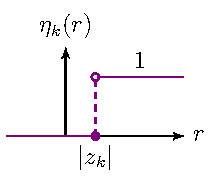
\includegraphics{Figuras/função salto.pdf} 
    \end{tabular}
    
    Então $n_f(r) = \dis{\sum_{k=1}^{N} \eta_k(r)}$. Segue que
    %
    \begin{align*}
        \sum_{k=1}^{N}\int_{|z_K|}^{R} \, \frac{dr}{r} 
        &= \sum_{k=1}^{N}\int_{|z_K|}^{R}\eta_k(r) \, \frac{dr}{r} \\
        &= \int_{|z_K|}^{R}\left(\sum_{k=1}^{N}\eta_k(r)\right) \, \frac{dr}{r} \\
        &= \int_{0}^{R}n_f(r) \, \frac{dr}{r}.
    \end{align*}
    %
    \end{proof}
    %
%\subsection{Ordem de crescimento e o número de zeros de uma função}
    % Agora, vamos usar a fórmula de Jensen para encontrar uma relação entre a
    % taxa de crescimento de uma função inteira no infinito e o comportamento
    % assintótico do número de zeros (contados com multiplicidade) desta
    % função dentro dos discos $D(0,R)$ quando $R\to +\infty$.
    
    % Primeiro, note que podemos reescrever a fórmula de Jensen da seguinte forma:
    % %
    % \begin{align*}
    %     \ln|f(0)| = \sum_{j=1}^n \ln\left|\frac{z_j}{R}\right| 
    %     + \frac{1}{2\pi}\int_0^{2\pi} \ln|f(Re^{i\theta})| \, d\theta,
    % \end{align*}
    % %
    % usando as propriedades do logaritmo e do valor absoluto.
    
    % Seja $f:U\subset\C\to\C$ é uma função holomorfa em $\overline{D(0,R)}$.
    % Para cada $r\in (0,R)$ denotamos por $n_f(r) \equiv n(r)$ o número de zeros 
    % de $f$, contados com multiplicidade, dentro do disco aberto $D(0,r)$.
    % Note que segue diretamente da definição que se $0 < r_1 \leq r_2 < R$, então
    % $n_f(r_1) \leq n_f(r_2)$, ou seja, $n_f$ é uma função não-decrescente. Usaremos
    % esse fato no seguinte lema que, por sua vez, será o primeiro de dois resultados
    % que nos permitirão extrair a relação entre zeros e a ordem de uma função.
    %
    % \begin{lema}
    % \label{lema:int-num-zeros}
    %     Sejam $R > 0$, $U\subseteq\C$ tal que $\overline{D(0,R)} \subseteq U$
    %     e $f:U\to\C$ uma função holomorfa. Se $z_1, z_2, \dots, z_n$ são zeros
    %     de $f$ em $D(0,R)$, então
    %     %
    %     \begin{equation*}
    %         \int_0^R n_f(r) \, \frac{dr}{r} 
    %         = \sum_{j=1}^n \ln\left|\frac{R}{z_j}\right|.
    %     \end{equation*}
    %     %
    % \end{lema}
    % %
    % \begin{proof}
    %     Note, primeiramente, que
    %     %
    %     \begin{equation*}
    %         \sum_{j=1}^n \ln\left|\frac{R}{z_j}\right| 
    %         = \sum_{j=1}^n \int_{|z_j|}^R \frac{1}{r} \, dr.
    %     \end{equation*}
    %     %
    %     Ademais, para cada $j=1, 2, \dots, n$, considere a função $\eta_j:\R\to\R$
    %     definida anteriormente:
    %     %
    %     \begin{equation*}
    %         \eta_j(r) 
    %         = \begin{cases}
    %         1, & |z_j| < r \\
    %         0, & |z_j| \geq r
    %         \end{cases}.
    %     \end{equation*}
    %     Daí, para cada $r$ fixado, temos
    %     %
    %     \begin{equation*}
    %         \sum_{j=1}^n \eta_j(r) = n_f(r),
    %     \end{equation*}
    %     %
    %     donde segue que
    %     %
    %     \begin{align*}
    %         \sum_{j=1}^n \int_{|z_j|}^R 1 \, \frac{dr}{r}
    %         = \sum_{j=1}^n \int_{0}^R \eta_j(r) \, \frac{dr}{r}
    %         = \int_{0}^R \left( \sum_{j=1}^n \eta_j(r) \right) \, \frac{dr}{r}
    %         = \int_{0}^R n_f(r) \, \frac{dr}{r},
    %     \end{align*}
    %     %
    %     como desejado.
    % \end{proof}
    %
    
    O segundo resultado que precisaremos é consequência imediata do 
    Corolário \ref{corol:num-zeros}.
    %
    \begin{corolario}
    \label{corol:jensen-com-zeros}
        Sejam $f:\C\to\C$ uma função inteira e $R>0$. Suponha que $f(0)\neq 0$
        e que $f(z)\neq 0$ para todo $z\in\partial D(0,R)$. Então
        %
        \begin{equation*}
            \int_0^R n_f(r) \, \frac{dr}{r}
            = \frac{1}{2\pi} \int_0^{2\pi} \ln|f(Re^{i\theta})| \, d\theta
            - \ln|f(0)|.
        \end{equation*}
        %
    \end{corolario}
    %
    \begin{proof}
       Pelo Corolário \ref{corol:num-zeros}, temos
       %
       \begin{equation*}
           \int_0^R n_f(r) \, \frac{dr}{r} 
           = \sum_{j=1}^n \ln\left|\frac{R}{z_j}\right|.
       \end{equation*}
       %
       Daí, basta usar esta identidade na fórmula de Jensen para obter o resultado.
    \end{proof}
    %
    \subsection{Funções de Ordem Finita}
    %
    \begin{definicao}
    \label{def:ordem-func}
        Seja $f:\C\to\C$ uma função inteira. Se existem um número positivo $\rho$
        e constantes $A,B>0$ tais que
        %
        \begin{equation*}
            |f(z)| \leq A\exp(B|z|^{\rho}), \forall z\in\C,
        \end{equation*}
        %
        dizemos que $f$ tem ordem de crescimento no máximo $\rho$. Definimos a
        ordem de crescimento de $f$ como sendo o número
        %
        \begin{equation*}
            \rho_f \equiv 
            \inf \left\{ \rho > 0 : 
            |f(z)| \leq A\exp(B|z|^{\rho}), \forall z\in\C \right\}.
        \end{equation*}
        %
    \end{definicao}
    %
    Alguns exemplos são:
    %
    \begin{itemize}
        \item a função $f:\C\to\C$ dada por $f(z) = e^z$ tem ordem de crescimento 1;
        \item a função $g:\C\to\C$ dada por $g(z) = e^{\alpha z^2 + z}, \alpha\in\C^*$
        tem ordem de crescimento 2;
        \item a função $f:\C\to\C$ dada por $f(z) = e^{e^z}$ não tem ordem de
        crescimento finita.
    \end{itemize}
    %
    \begin{teorema}
    \label{teo:est-num-zeros}
        Se $f:\C\to\C$ tem ordem de crescimento no máximo $\rho$, então:
        %
        \begin{enumerate}[(i)]
            \item $n_f(r) \leq Cr^{\rho}$ para algum $C>0$ e $r\gg 1$;
            \item se $z_1, z_2, \dots$ denotam os zeros de $f$, com $z_k\neq 0$,
            então para todo $s > \rho$ temos
            %
            \begin{equation*}
                \sum_{k=1}^{\infty} \frac{1}{|z_k|^2} < + \infty.
            \end{equation*}
            %
        \end{enumerate}
        %
    \end{teorema}
    %
    \begin{proof}
       Comecemos demonstrando (i). Observe que basta mostrar que vale a estimativa
       %
       \begin{equation*}
           n_f(r) \leq Cr^{\rho}
       \end{equation*}
       %
       no caso em que $f$ não se anula na origem. De fato, se $f(0) = 0$ e $k$
       é a multiplicidade de $0$, então a função $F:\C^*\to\C$ dada por 
       $F(z) = f(z)/z^k$ admite uma extensão inteira que não se anula na origem
       e tal que $n_F(r) = n_f(r) - k$. Logo,
       %
       \begin{align*}
           n_f(r) = n_F(r) + k &\leq Cr^{\rho} + k \\
                               &\leq Cr^{\rho} + kr^{\rho} \\
                               &= (C+k) r^{\rho},
       \end{align*}
       %
       usando o fato que $r\gg 1$. Dito de outro modo, se $f$ se anula na origem
       apenas mudamos o fator constante em $r^{\rho}$.
       
       Já que estamos assumindo que $f(0) \neq 0$, podemos aplicar o 
       Corolário \ref{corol:jensen-com-zeros}, que diz que
       %
       \begin{equation*}
           \int_0^R n_f(x) \, \frac{dx}{x} 
           = \frac{1}{2\pi} \int_0^{2\pi} \ln|f(Re^{i\theta})| \, d\theta - \ln|f(0)|.
       \end{equation*}
       %
       Escolhendo $R = 2r$ temos, pelas propriedades da integral, que
       %
       \begin{align*}
           \int_r^{2r} n_f(x) \, \frac{dx}{x}
           \leq \int_0^{2r} n_f(x) \, \frac{dx}{x}
           = \frac{1}{2\pi} \int_0^{2\pi} \ln|f(2re^{i\theta})| \, d\theta - \ln|f(0)|.
       \end{align*}
       %
       Lembrando que $n_f$ é monótona não-decrescente, temos a seguinte estimativa:
       %
       \begin{align*}
           \int_r^{2r} n_f(x) \, \frac{dx}{x}
           \geq n_f(r) \int_r^{2r} \frac{dx}{x} 
           = n_f(r)[\ln(2r) - \ln(r)]
           = n_f(r)\ln(2).
       \end{align*}
       %
       Por outro lado,
       %
       \begin{align*}
           \left| \frac{1}{2\pi} \int_0^{2\pi} \ln|f(2re^{i\theta})| \, d\theta \right|
           &\leq \frac{1}{2\pi} \int_0^{2\pi} |\ln|f(2re^{i\theta})| | \, d\theta \\
           &\leq \frac{1}{2\pi} \int_0^{2\pi} \ln\left(Ae^{B(2r)^{\rho}}\right) 
           \, d\theta \\
           &= \ln A + B2^{\rho}r^{\rho} \\
           &\leq r^{\rho}\ln A + B2^{\rho}r^{\rho} \\
           &= (\ln A + 2^{\rho}B)r^{\rho}.
       \end{align*}
       %
       Usando essas duas estimativas e tomando $r\gg 1$ suficientemente grande,
       temos
       %
       \begin{align*}
           n_f(r)\ln(2) &\leq \int_r^{2r} n_f(x) \, \frac{dx}{x} \\
                        &\leq \int_0^{2r} n_f(x) \, \frac{dx}{x} \\
                        &= \frac{1}{2\pi}\int_0^{2\pi} \ln|f(2re^{i\theta})| \, d\theta
                        - \ln|f(0)| \\
                        &\leq (\ln A + 2^{\rho}B)r^{\rho} + |\ln|f(0)|| \\
                        &\leq (\ln A + 2^{\rho}B)r^{\rho} + |\ln|f(0)||r^{\rho} \\
                        &= [\ln A + 2^{\rho}B + |\ln|f(0)||]r^{\rho},
       \end{align*}
       %
       donde segue que
       %
       \begin{equation*}
           n_f(r) \leq \frac{\ln A + 2^{\rho}B + |\ln|f(0)||}{\ln(2)}r^{\rho} 
           \equiv Cr^{\rho}.
       \end{equation*}
       %
       Agora, para o item 2, observe que
       %
       \begin{align*}
           \sum_{\substack{k\in\N \\ |z_k|\geq 1}} \frac{1}{|z_k|^s}
           &= \sum_{j=0}^{\infty} 
           \sum_{\substack{k\in\N \\ 2^j \leq |z_k| < 2^{j+1}}} \frac{1}{|z_k|^s} \\
           &\leq \sum_{j=0}^{\infty} \frac{1}{2^{sj}}n_f(2^{j+1}) \\
           &\leq \sum_{j=0}^{\infty} \frac{C}{2^{sj}}(2^{j+1})^{\rho} \\
           &\leq C2^{\rho} \sum_{j=0}^{\infty} 2^{(\rho - s)j} \\
           &< + \infty \text{ se } \rho < s.
       \end{align*}
       %
    \end{proof}
    %
    
    Esse teorema merece alguns comentários. Primeiro, é importante observar que
    a demonstração do item (ii) se aproveita de uma certa invariância por escala
    que é logarítmica. Além disso, uma pergunta natural em relação ao item
    (i) seria: podemos fazer melhor, isto é, existe uma estimativa mais forte para
    $n_f(r)$? A reposta é não, e o motivo fica claro nos seguintes exemplos.
    %
    \begin{exemplo}
        Considere a função $f:\C\to\C$ dada por $f(z) = \sen(\pi z)$, que tem
        zeros de ordem 1 nos inteiros. Ora, já que
        %
        \begin{align*}
            f(z) = \frac{e^{i\pi z} - e^{-i\pi z}}{2i},
        \end{align*}
        %
        temos que
        %
        \begin{align*}
            |f(z)| &\leq \frac{1}{2}\left( |e^{i\pi z}| + |e^{-i\pi z}| \right) \\
                   &\leq \frac{1}{2}\left( e^{\pi y} + e^{-\pi y} \right) \\
                   &\leq \frac{1}{2}\left( e^{\pi |z|} + e^{\pi |z|} \right) \\
                   &= e^{\pi |z|},
        \end{align*}
        %
        o que mostra que a ordem de crescimento de $f$ é no máximo 1. Por outro lado,
        tomando $z = ix$, podemos observar que
        %
        \begin{align*}
            |f(z)|=|f(ix)|&=\frac{1}{2}\left| e^{i\pi (ix)} - e^{-i\pi (ix)} \right| \\
                          &= \frac{1}{2}\left| e^{-\pi x} - e^{\pi x} \right| \\
                          &= \frac{1}{2} \left( e^{\pi x} - e^{-\pi x} \right) \\
                          &= \frac{1}{2}\left( 1 - e^{-2\pi x} \right)e^{\pi x} \\
                          &\geq \frac{1}{2}\left( 1 - e^{-2\pi} \right)e^{\pi x} \\
                          &= ce^{\pi |z|}.
        \end{align*}
        %
        Logo, $f$ tem ordem de crescimento $\rho = 1$. Daí, sendo
        %
        \begin{equation*}
            \mathcal{Z}(f) \equiv \{ z\in\C : f(z) = 0 \} = \mathbb{Z},
        \end{equation*}
        %
        temos, pelo teorema anterior,
        %
        \begin{align*}
            \sum_{k\in\mathbb{Z}^*} \frac{1}{|k|^s} 
            = \sum_{k=1}^{\infty} \frac{1}{|z_k|^s} < +\infty \text{ se } 1 = \rho < s.
        \end{align*}
        %
    \end{exemplo}
    %
    \begin{exemplo}
        Considere a função inteira $f:\C\to\C$ dada por
        %
        \begin{equation*}
            f(z) = \cos(z^{1/2}) \equiv \sum_{n=0}^{\infty} (-1)^n \frac{z^n}{(2n)!}.
        \end{equation*}
        %
        Note que não estamos falando da composta da função cosseno com o ramo
        principal da raiz quadrada, apesar da notação. Podemos pensar $f$ como
        continuação analítica dessa composta.
        
        Lembrando que
        %
        \begin{equation*}
            \cos z = \frac{e^{iz} + e^{-iz}}{2}
        \end{equation*}
        %
        e que $|e^z| \leq e^{|z|}$, temos
        %
        \begin{align*}
            |f(z)| &= \frac{1}{2}\left| 
            e^{i\exp\left(\frac{1}{2}(\ln|z| + i\arg z)\right)} 
            + e^{-i\exp\left(\frac{1}{2}(\ln|z| + i\arg z)\right)} \right| \\
            &= \frac{1}{2}\left| e^{i|z|^{1/2}\exp(i\arg z/2)} 
            + e^{-i|z|^{1/2}\exp(i\arg z/2)} \right| \\
            &\leq e^{ \left| i|z|^{1/2}\exp(i\arg z/2) \right| } \\
            &= e^{|z|^{1/2}}.
        \end{align*}
        %
        Portanto, $f$ tem crescimento no máximo $1/2$. Note que $f$ se anula em
        $z_n = \dis \left( (n+1/2)\pi \right)^2 $ e, ademais, a série
        %
        \begin{equation*}
            \sum_{n\in\mathbb{Z}^*} \frac{1}{|z_n|^s} < +\infty \text{ se } s > 1/2.
        \end{equation*}
        %
    \end{exemplo}
    %
    Uma outra pergunta interessante é: existe alguma função inteira cujos zeros são
    dados exatamente pela lista $z_1, z_2, \dots$, contados com multiplicidade? Dito
    de outro modo: dada uma lista de números complexos, conseguimos encontrar uma 
    função inteira cujos zeros são exatamente aqueles números?
    
    O ``candidato natural'', pensando em polinômios, seria
    %
    \begin{equation*}
        f(z) = \lim_{n\to\infty} (z-z_1)(z-z_2)\cdots(z - z_n),
    \end{equation*}
    %
    mas esse produto é complicado de controlar, pois a cada novo valor de $n$ não
    só temos uma nova parcela quando abrimos esse produto, mas mudamos as parcelas
    anteriores.
    
    Weierstrass mostrou como inserir fatores adequados nesse candidato de modo que
    possamos construir um produto semelhante mas que seja convergente e de forma que
    nenhum novo zero apareça no processo. Trataremos disto na seção a seguir.
    
\section{Produtos Infinitos}

    Dada uma sequência $\{ a_n \}_{n\in\N}$ de números complexos, dizemos que o
    produto $\dis{ \prod_{n=1}^{\infty} (1+a_n) }$ converge se
    %
    \begin{equation*}
        \lim_{n\to\infty} \prod_{j=1}^n (1+a_j)
    \end{equation*}
    %
    converge. A parcela 1 pode parecer artificial a priori, mas ela se torna
    natural quando lembramos que 1 é o elemento neutro da multiplicação.
    %
    \begin{proposicao}
    \label{prop:prod-inf}
        Se $\dis{\sum_{n\in\N} |a_n| < +\infty }$, então o produto
        $\dis{ \prod_{n=1}^{\infty} (1+a_n) }$ converge. Ademais, o produto converge
        para zero se, e somente se, um de seus fatores é nulo, ou seja, existe
        $k\in\N$ tal que $1+a_k = 0$.
    \end{proposicao}
    %
    \begin{proof}
       Se $\dis{\sum_{n\in\N} |a_n| < +\infty }$, então existe $n_0\in\N$
       tal que se $n\geq n_0$ então $|a_n| < 1/2$. Para simplificar o 
       argumento, vamos supor que esta desigualdade é válida para todo $n\in\N$.
       
       Considere o ramo principal do logaritmo e a sequência $\log(1+a_n)$.
       É claro que se $|z| < 1/2$, então
       %
       \begin{equation*}
           1 + z = e^{\log(1+z)}.
       \end{equation*}
       %
       Portanto, os produtos parciais podem ser escritos como
       %
       \begin{equation*}
           \prod_{j=1}^n (1 + a_j) = \prod_{j=1}^n e^{\log(1 + a_j)} = e^{B_n},
       \end{equation*}
       %
       sendo
       %
       \begin{equation*}
           B_n = \sum_{j=1}^n \underbrace{\log(1 + a_j)}_{b_j}.
       \end{equation*}
       %
       Usando expansão em série de potências, temos que
       %
       \begin{align*}
           |\log(1+w)|&=\left| \sum_{n=0}^{\infty} (-1)^n \frac{w^{n+1}}{n+1} \right| \\
                      &\leq |w|\cdot\left| 1 - \frac{w}{2} + \frac{w^2}{3} 
                      - \cdots \right| \\
                      &\leq |w|\cdot\frac{1}{1 - |w|} \\
                      &\leq 2|w|,
       \end{align*}
       %
       considerando $|w| \leq 1/2$. Portanto,
       %
       \begin{equation*}
           |B_n| = \left| \sum_{j=1}^n \log(1 + a_j) \right| 
           \leq \sum_{j=1}^n |\log(1+a_j)|
           \leq \sum_{j=1}^n 2|a_j|,
       \end{equation*}
       %
       ou seja, $B_{\infty}$ é absolutamente convergente, isto é, existe
       $B\in\C$ tal que $B_n \xrightarrow{n\to\infty} B$. Ora, já que
       %
       \begin{equation*}
           \prod_{j=1}^n (1+a_n) = e^{B_n},
       \end{equation*}
       %
       segue que existe
       %
       \begin{equation*}
           \lim_{n\to\infty} \prod_{j=1}^n (1+a_n) = \lim_{n\to\infty} e^{B_n} = e^B.
       \end{equation*}
       %
       Por fim, observe que se $1+a_n \neq 0 \, \forall n\in \N$, então
       %
       \begin{equation*}
           \left| \prod_{j=1}^{\infty} (1+a_j) \right| = |e^B| \neq 0.
       \end{equation*}
       %
    \end{proof}
    %
    
    O próximo passo é falar de produtos infinitos de funções holomorfas.
    %
    \begin{proposicao}
    \label{prop:prod-inf-func-holom}
        Suponha que $\{ F_n \}_{n\in\N}$ é uma sequência de funções complexas
        definidas em um domínio $\Omega\subseteq\C$. Se existem constantes
        $c_n>0$ tais que $\dis{ \sum_{n\in\N} x_n < +\infty }$ e 
        $|F_n(z) - 1| \leq c_n \, \forall n\in\N$ e $\forall z\in\Omega$, então
        %
        \begin{enumerate}[(i)]
            \item o produto $\dis{ \prod_{n=1}^{\infty} F_n(z) }$ converge
            uniformemente em $\Omega$ para alguma função holomorfa em $F(z)$;
            \item se $F_n(z) \neq 0 \, \forall z\in\Omega$ para cada $n\in\N$, 
            então $\dis{ \frac{F'(z)}{F(z)} = 
            \sum_{n=1}^{\infty} \frac{F_n'(z)}{F_n(z)} }$.
        \end{enumerate}
        %
    \end{proposicao}
    %
    \begin{proof}
       Vamos começar com (i). Note que para cada $z\in\Omega$ fixado podemos
       escrever $F_n(z) = 1 + a_n(z)$. Ademais, segue da hipótese que
       $|a_n(z)| = |F_n(z) - 1| \leq c_n$ e que
       %
       \begin{equation*}
           \sum_{n\in\N} |a_n(z)| \leq \sum_{n\in\N} c_n < +\infty.
       \end{equation*}
       %
       Logo, existe
       %
       \begin{equation*}
           \lim_{n\to\infty} \prod_{j=1}^n F_j(z) 
           = \lim_{n\to\infty} \prod_{j=1}^n [1 + a_j(z)].
       \end{equation*}
       %
       Além disso, os produtos parciais de $F_j$ convergem uniformemente, uma vez
       que sendo $D' = \dis{ D\left( 0, 2\sum_{n\in\N} c_n \right) }$, temos
       %
       \begin{align*}
           \left| \prod_{j=1}^{m+n} F_j(z) - \prod_{j=1}^{n} F_j(z) \right|
           &=\left|\prod_{j=1}^{m+n} [1+a_j(z)] - \prod_{j=1}^{n} [1+a_j(z)] \right| \\
           &= \left| e^{B_{m+n}(z)} - e^{B_n(z)} \right| \\
           &= \left| \int_{B_n(z)}^{B_{m+n}(z)} e^w \, dw \right| \\
           &\leq \sup_{w\in D'} 
           |e^w|\cdot |B_{m+n}(z) - B_n(z)| \\
           &= k|B_{m+n} - B_n(z)| \xrightarrow{m,n\to\infty} 0.
       \end{align*}
       %
       Logo, a função
       %
       \begin{equation*}
           z \mapsto \lim_{n\to\infty} \prod_{j=1}^n F_j(z) 
                                       \equiv \prod_{j=1}^{\infty} F_j(z)
                                       \equiv F(z)
       \end{equation*}
       %
       é holomorfa em $\Omega$.
       
       Agora, para o item (ii), seja $K\subseteq\Omega$ um subconjunto compacto
       e defina
       %
       \begin{equation*}
           G_n(z) = \prod_{j=1}^n F_j(z), \forall z\in\Omega.
       \end{equation*}
       %
       Já que $G_n \xrightarrow[\text{unif}]{n\to\infty} F$, temos que
       $G_n' \xrightarrow[\text{unif em compactos}]{n\to\infty} F'$.
       Para ver isto basta observar que
       %
       \begin{equation*}
           G_n'(z) - F'(z) = 
           \frac{1}{2\pi i} \int_{\y} (G_n(w) - F(w))\frac{1}{(w-z)^2} \, dw
       \end{equation*}
       %
       sendo $\y$ como ilustrado abaixo.
       %
       \begin{figure}[H]\centering
           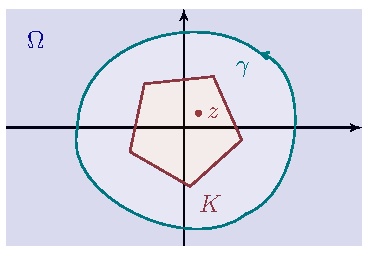
\includegraphics{Figuras/y para Gn'-Fn'.pdf}
       \end{figure}
       %
       Por hipótese, $F_n(z) \neq 0$ para todos $n\in\N$ e $z\in\Omega$, de modo
       que $F(z)\neq 0$ para todo $z\in\Omega$. Já que $F$ é holomorfa e, 
       consequentemente, contínua, podemos dizer que
       %
       \begin{equation*}
           \inf_{z\in K} |F(z)| = F(z_*) > 0.
       \end{equation*}
       %
       Portanto, podemos garantir que $G_n(z)$ é uniformemente limitada inferiormente
       em $n$ e $z\in K$. De fato,
       %
       \begin{align*}
           \inf_{z\in K} |G_n(z)| = \inf_{z\in K} |G_n(z) - F(z) + F(z)|
           \geq \inf_{z\in K} | |G_n(z) - F(z)| - |F(z)| |.
       \end{align*}
       %
       Como $G_n$ converge uniformemente para $F$, existe $n_0\in\N$ tal que
       se $n\geq n_0$, então 
       $|G_n(z) - F(z)| < \dis{\frac{1}{2} F(z_*) }$ para todo 
       $z\in K$. Logo, para todo $n\geq n_0$ temos
       %
       \begin{equation*}
           \inf_{z\in K} |G_n(z)| > \frac{1}{2}\inf_{z\in K} |F(z)| 
                                  = \frac{1}{2} F(z_*) > 0.
       \end{equation*}
       %
       Por outro lado, se $n\leq n_0$, então como $F_j(z)\neq 0$ para todo 
       $z\in\Omega$, temos que
       %
       \begin{align*}
           \inf_{z\in K} |G_n(z)| &= \inf_{z\in K} |F_1(z)|\cdots|F_n(z)| \\
                                  &\geq \prod_{j=1}^n \inf_{z\in K} |F_j(z)| \\
                                  &= |F_1(z^1_*)| \cdots |F_n(z^n_*)| \equiv I_K.
       \end{align*}
       %
       Portanto, 
       %
       \begin{equation*}
           \inf_{n\in\N} \inf_{z\in K} |G_n(z)| 
           \geq \min\left\{ I_K, \frac{1}{2}|F(z_*)| \right\} > 0,
       \end{equation*}
       %
       donde segue que 
       %
       \begin{equation*}
           \frac{G_n'}{G_n} \xrightarrow[\text{unif. em } K]{n\to\infty} \frac{F'}{F}
       \end{equation*}
       %
       para cada $z\in K$ e, como $K$ é compacto arbitrário, segue que
       %
       \begin{equation*}
           \frac{G_n'(z)}{G_n(z)} \xrightarrow{n\to\infty} \frac{F'(z)}{F(z)}
       \end{equation*}
       %
       para cada $z\in\Omega$. Observe que não podemos garantir que essa última
       convergência é uniforme em $\Omega$.
       
       Ademais, para cada $n\in\N$ temos
       %
       \begin{align*}
           \frac{G_n'(z)}{G_n(z)} 
           &= \frac{ \frac{d}{dz}[F_1(z)\cdots F_n(z)] }{F_1(z)\cdots F_n(z)} \\
           &= \sum_{j=1}^n F'_j(z)
           \frac{F_1(z)\cdots F_{j-1}(z)F_{j+1}(z)\cdots F_n(z)}{F_1(z)\cdots F_n(z)} 
           \\
           &= \sum_{j=1}^n \frac{F'_j(z)}{F_j(z)},
       \end{align*}
       %
       o que mostra que
       %
       \begin{equation*}
           \frac{F'(z)}{F(z)} = \lim_{n\to\infty} \frac{G'_n(z)}{G_n(z)}
                              = \lim_{n\to\infty} \sum_{j=1}^n \frac{F'_j(z)}{F_j(z)}
                              \equiv \sum_{j=1}^{\infty} \frac{F'_j(z)}{F_j(z)}.
       \end{equation*}
       %
    \end{proof}
    %
    
    Vamos usar este teorema para trabalhar com um exemplo interessante.
    \begin{exemplo}[A fórmula do produto da função seno]
        Vamos estabelecer a validade da seguinte fórmula:
        %
        \begin{equation*}
            \frac{\sen(\pi z)}{\pi} = z\prod_{n=1}^{\infty} 
            \left( 1 - \frac{z^2}{n} \right).
        \end{equation*}
        %
        Para tanto, vamos estabelecer uma fórmula para $\cot(\pi z)$.
        Apesar de parecer estranha, a escolha da função cotangente é tudo menos
        coincidência. De fato, devido à Proposição \ref{prop:prod-inf-func-holom},
        para encontrar uma fórmula do produto da função $\sen(\pi z)/\pi$ precisaremos 
        considerar a sua derivada logarítmica, que nada mais é que $\pi\cot(\pi z)$.
        
        Vamos então mostrar que, para todo $z\in\C\setminus\mathbb{Z}$, temos
        %
        \begin{equation*}
            \pi\cot(\pi z) = \sum_{n=-\infty}^{\infty} \frac{1}{z+n}
                           \equiv \lim_{n\to\infty} \sum_{|j|\leq n} \frac{1}{z+j}
                           = \frac{1}{z} + \sum_{n=1}^{\infty} \frac{2z}{z^2 - n^2},
        \end{equation*}
        %
        onde usamos que
        %
        \begin{equation*}
            \frac{1}{z+n} + \frac{1}{z-n} = \frac{2z}{z^2 - n^2}.
        \end{equation*}
        %
        A estratégia para mostrar essa identidade será mostrar que tanto
        $F(z) = \pi\cot(\pi z)$ e $S(z) = \dis{\frac{1}{z} + 
        \sum_{n=1}^{\infty} \frac{2z}{z^2- n^2}}$ satisfazem as seguintes propriedades:
        %
        \begin{enumerate}[(i)]
            \item $H(z+1) = H(z)$;
            \item $H(z) = \dis{ \frac{1}{z} + H_0(z) }$, sendo $H_0$ analítica próxima
            do zero;
            \item $H(z)$ tem polos simples em $\Z$ e nenhuma outra singularidade.
        \end{enumerate}
        %
        De fato, para $F$,
        %
        \begin{enumerate}[(i)]
            \item 
            %
            \begin{align*}
                F(z+1)=\pi\cot(\pi(z+1)) &= \pi\frac{\cos(\pi(z+1))}{\sen(\pi(z+1))} \\
                                         &= \pi\frac{-\cos(\pi z)}{-\sen(\pi z)} \\
                                         &= \pi\cot(\pi z) \\
                                         &= F(z).
            \end{align*}
            %
            \item 
            %
            \begin{align*}
                \lim_{z\to 0} zF(z) &= \lim_{z\to 0} \pi z 
                \frac{\cos(\pi z)}{\sen(\pi z)} \\
                &= \lim_{z\to 0} \cos(\pi z)\cdot\frac{\pi z}{\sen(\pi z)} \\
                &= \lim_{z\to 0} \frac{\pi z}{\sen(\pi z)} \\
                &= 1 = \res(F,0).
            \end{align*}
            %
            Como $F$ tem apenas singularidades isoladas em $\Z$, segue do
            teorema de Laurent que para todo $z\in A(0,0,1)$ temos
            %
            \begin{equation*}
                F(z) = \frac{\res(F,0)}{z} + H_0(z) = \frac{1}{z} + H_0(z),
            \end{equation*}
            %
            com $H_0$ holomorfa em $D(0,1).$
            
            \item $F$ é claramente holomorfa em $\C\setminus\Z$.
        \end{enumerate}
        %
        Agora, para $S$, temos
        %
        \begin{enumerate}[(i)]
            \item $\forall z\in\C\setminus\Z$:
            %
            \begin{align*}
                S(z+1) &= \lim_{n\to\infty} \sum_{|j|\leq n} \frac{1}{z+1+j} \\
                       &= \lim_{n\to\infty}\left( \sum_{|j|\leq n+1} \frac{1}{z+j}
                       - \frac{1}{z-n-1} - \frac{1}{z-n} \right) \\
                       &= \lim_{n\to\infty} \sum_{|j|\leq n} \frac{1}{z_j} \\
                       &= S(z)
            \end{align*}
            %
            \item $\forall z\in D(0,1/2)$, temos
            %
            \begin{equation*}
                S(z) = \frac{1}{z} + \sum_{n=1}^{\infty} \frac{2z}{z^2 - n^2}.
            \end{equation*}
            %
            Considere a sequência de funções $h_n:D(0,1/2)\to\C$ dada por
            $h_n(z) = \dis{ \frac{2z}{z^2 - n^2} }$. Para cada $n\in\N$, temos
            que $h_n$ é uma função holomorfa e, além disso,
            %
            \begin{align*}
                \sup_{z\in D(0,1/2)} |h_n(z)| 
                = \sup_{z\in D(0,1/2)} \left| \frac{2z}{n^2
                \left( \frac{z^2}{n^2} - 1 \right)} \right|
                = \frac{2}{n^2}\sup_{z\in D(0,1/2)} 
                \frac{|z|}{\left| \frac{z^2}{n^2} - 1 \right|}
                = \frac{2}{n^2}.
            \end{align*}
            %
            Logo,
            %
            \begin{equation*}
                \sum_{n=1}^{\infty} \sup_{z\in D(0,1/2)} |h_n(z)|
                \leq 2\sum_{n=1}^{\infty} \frac{1}{n^2} < +\infty.
            \end{equation*}
            %
            Pelo teste M de Weierstrass, segue que 
            $\dis{ \sum_{n=1}^{\infty} h_n(z) \equiv S_0(z) }$ define uma função
            $S_0: D(0,1/2) \to\C$ holomorfa. Assim, 
            %
            \begin{equation*}
                S(z) = \frac{1}{z} + S_0(z),
            \end{equation*}
            %
            com $S_0$ holomorfa em $D(0,1/2)$.
            
            \item Fixado $n\in\Z$, temos que
            %
            \begin{align*}
                S(z) &= \frac{1}{z} + \sum_{j\in\N\setminus\{n\}} \frac{2z}{z^2 - j^2}
                + \frac{2z}{z^2 - n^2} \\
                &= S_1(z) + \frac{1}{z+n} + \frac{1}{z-n}.
            \end{align*}
            %
            Pelo teste M de Weierstrass, segue que $S_1(z) + \dis{\frac{1}{z+n}}$
            é holomorfa em $D(n, 1/2)$, de modo que $S$ tem apenas polos simples
            em cada ponto de $\Z$.
        \end{enumerate}
        %
        Sabendo que $F$ e $S$ satisfazem (i), (ii) e (iii), podemos afirmar que
        $H:\C\setminus\Z\to\C$ dada por
        %
        \begin{equation*}
            H(z) \equiv F(z) - S(z)
        \end{equation*}
        %
        satisfaz $H(z+1) = H(z)$. Ademais, segue da propriedade (ii) que
        $\res(H,0) = 0$, de modo que $z=0$ é uma singularidade removível de $H$.
        Esta informação, junto com a periodicidade de $H$ dada pelo item (i)
        implica que, para todo $n\in\Z$,
        %
        \begin{equation*}
            \lim_{z\to n} H(z) = \lim_{z\to n} H(z-n) = \lim_{z\to 0} H(z) = 0.
        \end{equation*}
        %
        Logo, segue do teorema de Riemann que $H$ admite extensão inteira.
        
        Para estabelecer a fórmula da cotangente, é suficiente mostrar que
        $H$ é limitada e usar o teorema de Liouville.
        
        Ademais, para mostrar que $H$ é limitada, basta trabalhar na faixa
        %
        \begin{equation*}
            S_{\frac{1}{2}} = \left\{ z\in\C : |\Re(z)| \leq \frac{1}{2} \right\},
        \end{equation*}
        %
        uma vez que $H$ satisfaz a periodicidade (i).
        %
        \begin{figure}[H]\centering
            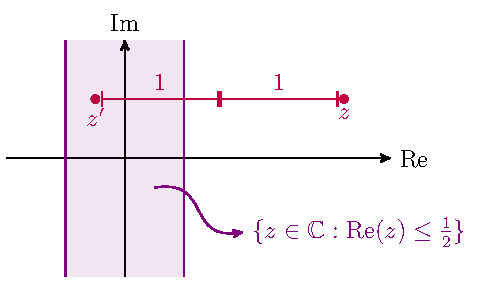
\includegraphics{Figuras/S_meio.pdf}
        \end{figure}
        %
        Já que $H:\C\to\C$ é inteira, então $H$ é limitada em
        %
        \begin{equation*}
            \Omega_1 = S_1 \cap S_{\frac{1}{2}},
        \end{equation*}
        %
        com
        %
        \begin{equation*}
            S_1 = \{ z\in\C : |\Im(z)| \leq 1 \},
        \end{equation*}
        %
        ou seja, 
        %
        \begin{equation}
            \sup_{z\in \Omega_1} |H(z)| = k_1 < +\infty
        \end{equation}
        %
        pois $\Omega_1$ é um compacto, como ilustrado abaixo.
        %
        \begin{figure}[H]\centering
            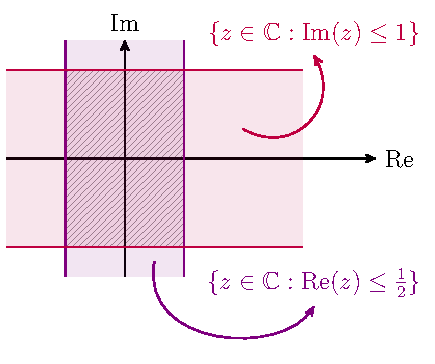
\includegraphics{Figuras/S_meio cap S_1.pdf}
            \caption{%
                A região hachurada, $\Omega_1$, é um compacto.
            }
        \end{figure}
        %
        Para terminar a demonstração que $H$ é limitada em $S_{\frac{1}{2}}$,
        resta analisar o que acontece com a função em
        %
        \begin{equation*}
            \Omega_2 = S_{\frac{1}{2}} \cap \left\{ z\in\C : |\Im(z)| > 1 \right\}.
        \end{equation*}
        %
        Ora, se $z = x+iy$, então
        %
        \begin{align*}
            \cot(\pi z) &= 
            i\frac{ e^{i\pi z} + e^{-i\pi z} }{ e^{i\pi z} - e^{-i\pi z} } \\
            &= i\frac{ e^{i\pi x}e^{-\pi y} + e^{-i\pi x}e^{\pi y} }
            { e^{i\pi x}e^{-\pi y} - e^{-i\pi x}e^{\pi y} } \\
            &= i\frac{ e^{-2\pi y} + e^{-2\pi ix} }{ e^{-2\pi y} - e^{-2\pi ix} }.
        \end{align*}
        %
        Como estamos supondo $|y|>1$, segue que
        %
        \begin{align*}
            |\cot(\pi z)| = 
            \left| 
            \frac{ e^{-2\pi y} + e^{-2\pi ix} }{ e^{-2\pi y} - e^{-2\pi ix} } 
            \right|
            \leq \frac{ 1 + e^{-2\pi y} }{ 1 - e^{-2\pi y} }
            \leq \widetilde{k_1}.
        \end{align*}
        %
        Ainda para $|y|>1$ e $|x|\leq 1/2$, temos
        %
        \begin{align*}
            \left| 
            \frac{1}{z} + \sum_{n=1}^{\infty} \frac{2z}{z^2 - n^2} 
            \right|
            &= \left| 
            \frac{1}{x+iy} + \sum_{n=1}^{\infty} \frac{2(x+iy)}{x^2 - y^2 - n^2 +2ixy} 
            \right| \\
            &\leq \frac{1}{\sqrt{x^2 + y^2}} 
            + \sum_{n=1}^{\infty} \frac{|2x|}{\sqrt{(x^2 - y^2 - n^2)^2 + 4x^2y^2}} \\
            &+ \sum_{n=1}^{\infty} \frac{|2y|}{\sqrt{(x^2 - y^2 - n^2)^2 + 4x^2y^2}} \\
            &\leq 1 
            + \sum_{n=1}^{\infty} \frac{1}{|y|^2 + n^2 - 1/4}
            + \sum_{n=1}^{\infty} \frac{|2y|}{|y|^2 + n^2 - 1/4} \\
            &\leq 1 + \sum_{n=1}^{\infty} \frac{1}{n^2} 
            + 2\sum_{n=1}^{\infty} \frac{|y|}{|y|^2/4 + n^2 - n^2/4} \\
            &\leq 1 + \frac{\pi^2}{6} + 
            8\sum_{n=1}^{\infty} \frac{|y|}{\frac{1}{4}(|y|^2 + 3n^2)} \\
            &\leq 1 + \frac{\pi^2}{6} +
            8\sum_{n=1}^{\infty} \frac{|y|}{|y|^2 + n^2}.
        \end{align*}
        %
        Agora, como $b:(0, +\infty)\to\R$ dada por $\dis{ b(x) = \frac{|y|}{|y|^2 + x^2} }$
        é decrescente já que
        %
        \begin{equation*}
            b'(x) = |y|\frac{-2x}{(|y|^2 + x^2)^2} < 0 \, \forall x+iy \in\Omega_2,
        \end{equation*}
        %
        podemos assegurar que
        %
        \begin{equation*}
            \sum_{n=1}^{\infty} \frac{|y|}{|y|^2 + n^2} 
            \leq
            \int_0^{\infty} \frac{|y|}{|y|^2 + x^2} \, dx.
        \end{equation*}
        %
        \begin{figure}[H]\centering
            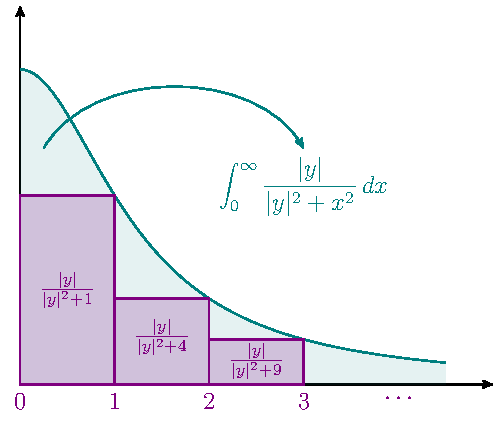
\includegraphics{%
                Figuras/majoração por integral.pdf
            }
        \end{figure}
        %
        Agora, considerando a mudança de variáveis $u = x/|y|$, temos
        %
        \begin{align*}
            \int_0^{\infty} \frac{|y|}{|y|^2 + x^2} \, dx = 
            \int_0^{\infty} \frac{1}{1 + u^2} \, du =
            \frac{\pi}{2}.
        \end{align*}
        %
        Até o momento, mostramos que
        %
        \begin{enumerate}
            \item $|\cot(\pi z)| = \dis{ 
            \left|\frac{ e^{-2\pi y} + e^{-2i\pi x} }{ e^{-2\pi y} - e^{-2i\pi x} } \right|
            \leq \frac{ 1 + e^{-2\pi y} }{ 1 - e^{-2\pi y} }
            \leq \widetilde{k_1}}$;
            
            \item $|S(z)| = \dis{ 
            \left| \frac{1}{z} + \sum_{n=1}^{\infty} \frac{2z}{z^2 - n^2} \right| 
            \leq 1 + \frac{\pi^2}{6} + 8\int_0^{\infty} \frac{|y|}{|y|^2 + x^2} \, dx
            = 1 + \frac{\pi^2}{6} + 4\pi =
            \widetilde{k_2}}$,
        \end{enumerate}
        %
        donde segue que
        %
        \begin{align*}
            \sup_{z\in\Omega_2} |H(z)| \leq 
            \sup_{z\in\Omega_2} |F(z) - S(z)| \leq
            \pi\widetilde{k_1} + \widetilde{k_2} \equiv
            k.
        \end{align*}
        %
        Portanto, lembrando que $H$ é periódica, temos
        %
        \begin{equation*}
            \sup_{z\in\C} |H(z)| =
            \sup_{z\in\Omega_1\cup\Omega_2} |H(z)| \leq
            k,
        \end{equation*}
        %
        ou seja, $H$ é limitada em $\C$.
        Pelo teorema de Liouville, como $H$ é inteira, temos
        $H(z)$ constante. 
        Agora, note que $H$ pode ser vista como extensão holomorfa de $F(z) - S(z)$,
        que é uma função ímpar. Portanto, $H$ também é ímpar e $H(0) = 0$, donde segue 
        que $H\equiv 0$, ou seja, $F(z) \equiv S(z)$ e temos
        %
        \begin{equation*}
            \pi\cot(\pi z) = \frac{1}{z} + \sum_{n=1}^{\infty} \frac{2z}{z^2 - n^2},
            \, \forall z\in\C\setminus\Z.
        \end{equation*}
        %
        Finalmente, para mostrar a fórmula de produto para o seno, sejam
        %
        \begin{align*}
            G(z) &= \frac{\sen(\pi z)}{\pi} , \\
            P(z) &= z\prod_{n=1}^{\infty} \left( 1 - \frac{z^2}{n^2} \right).
        \end{align*}
        %
        Para mostrar a convergência de $P(z)$, vamos usar a 
        Proposição \ref{prop:prod-inf-func-holom} com $P(z) = zF(z)$, 
        $\Omega = D(0,R)\setminus\Z$,
        $F_n(z) = 1 - \dis{ \frac{z^2}{n^2} }$. Daí, temos
        %
        \begin{equation*}
            |F_n(z) - 1| \leq \sup_{z\in\Omega} \frac{|z|^2}{n^2} = \frac{R^2}{n^2}
            \equiv c_n.
        \end{equation*}
        %
        Portanto, para todo $z\in\Omega$,
        %
        \begin{align*}
            \frac{P'(z)}{P(z)} =
            \frac{1}{z} + \sum_{n=1}^{\infty} \frac{ -\frac{2z}{n^2} }{ 1 - \frac{z^2}{n^2} }
            = \frac{1}{z} + \sum_{n=1}^{\infty} \frac{2z}{z^2 - n^2}.
        \end{align*}
        %
        Agora, como $G'(z)/G(z) = \pi\cot(\pi z)$, o resultado que acabamos de mostrar
        nos dá, para todo $z\in\Omega$,
        %
        \begin{equation*}
            \left( \frac{P(z)}{G(z)} \right)'
            = \frac{ P'(z)G(z) - P(z)G'(z) }{ G^2(z) }
            = \frac{P(z)}{G(z)}\left[ \frac{P'(z)}{P(z)} - \frac{G'(z)}{G(z)} \right]
            \equiv 0,
        \end{equation*}
        %
        de modo que $P(z) = cG(z)$ para alguma constante $c, \, \forall z\in\Omega$,
        pois $\Omega$ é conexo. 
        Ora, então
        %
        \begin{equation*}
            1 
            = \lim_{z\to 0} \prod_{n=1}^{\infty} \left( 1 - \frac{z^2}{n^2} \right)
            = \lim_{z\to 0} \frac{P(z)}{z} 
            = c\lim_{z\to 0} \frac{G(z)}{z}
            = c\lim_{z\to 0} \frac{\sen(\pi z)}{\pi z}
            = c,
        \end{equation*}
        %
        onde usamos que o produtório é holomorfo.
        Portanto, $P(z) = G(z)$ para todo $z\in\Omega$. Pelo Princípio da Identidade,
        como $\Omega$ é aberto e conexo, segue que essa identidade vale para todo
        $z\in\C$.
    \end{exemplo}
    
    \section{O Teorema de Weierstrass}
    
    Anteriormente, vimos que, para construir uma função com zeros prescritos na forma de uma lista ou sequência $\{a_n\}$, uma tentativa ingênua era escrever
    %
    $$ f(z) = \lim_{n \to \infty} (z-a_1) \cdots (z-a_n).$$
    %
    Produtos como esse (em geral) não convergem para qualquer sequência escolhida $\{a_n\}$, então essa não é a melhor escolha para construir $f$. 
    
    Mostramos, também, que vale a igualdade 
    %
    $$\frac{\sin{\pi z}}{\pi} = z \prod_{n = 1}^{\infty} \left(1 - \frac{z^2}{n^2}\right)$$
    %
    e a função $\sin{\pi z}$ se anula exatamente em $\mathbb{Z}$. Analizando o produto com mais cuidado, vamos que cada parcela é da forma $(n^2 - z^2)/n^2 = (n - z)(n + z)/n^2$ que se anula exatamente em $\pm n \in \Z$. A escolha do termo $z^2$ nas parcelas foi, então, boa. 
    
    além disso, o fato de termos escolhido fatores 
    %
    $$\left(1 - \frac{z^2}{n^2}\right)$$
    %
    em vez de $(n^2 - z^2)$ nos permitiu usar a Proposição \ref{prop:prod-inf-func-holom} de forma simples. 
    
    Se queremos definir uma função que se anula precisamente em uma sequência qualquer $\{a_n\}$ de uma forma análoga à vista acima, ter $z^2$ nos fatores pode não ser vantajoso, pois $-a_n$ pode não estar na sequência e mesmo assim anula a função. Portanto, pode ser um bom caminho considerar fatores da forma
    %
    $$ \left(1 - \frac{z}{a_n}\right)g_n(z), $$
    %
    onde $g_n(z)$ são funções que facilitariam a convergência. O grande problema está em como escolher tais funções e é neste ponto que reside a maior contribuição de Weierstrass, ele encontrou funções que garantem a convergência dada qualquer sequência $\{a_n\}$. 
    
    Vamos enunciar o grande resultado desta seção agora e demonstrá-lo no decorrer do texto.
    
    \begin{teorema}[Weierstrass]
        Dada uma sequência $\{a_n\}$ de números complexos tal que $|a_n| \to \infty$ conforme $n \to \infty$, existe uma função inteira $f: \C \to \C$ que se anula em todo $a_k$ e em nenhum outro ponto.
    \end{teorema}
    
    Note que é necessário que $|a_n| \xrightarrow{n\to\infty} \infty$, pois, do
    contrário, teríamos alguma subsequência $\{a_{n_k}\}$ de $\{a_n\}$ seria convergente
    e, pelo princípio da identidade, $f\equiv 0$, o que é absurdo, pois estamos assumindo que
    $f$ se anula apenas em $a_1, a_2, \dots$.
    
    %Fatores de weierstrass
    %estimativas
    %serie do log(1-z)...
    
    
    
    
    
    
    
    
    